%
%    18afmc template paper adapted from 14afmc template.
%
%    Format: LaTeX2e.
%
\documentclass[twocolumn]{afmc_art}
\usepackage{amsmath,defns}
\usepackage{url}
\usepackage{graphicx}
\usepackage{hyperref} 
\hypersetup{pdftex,
            backref=true,
            hyperindex=true,
            colorlinks=true,
            citecolor=blue,
            bookmarks=true,
            breaklinks=true}
\newcommand{\zs}{\zeta}
\newcommand{\uu}{{\bar u}}
\newcommand{\vv}{{\bar v}}
\newcommand{\bq}{{\bar q}}
\newcommand{\qq}{{\bar{\vec q}}}
\newcommand{\ee}{\textsc{e}}
\newcommand{\rnu}{R_\nu}
\newcommand{\ros}{{\dot\varepsilon}}
%
%%%  Fill in following information.
%
%%%%%%%%%%%%%%%%%%%%%%%%%%%%%%%%%%%%%%%%%%%%%%%%%%%%%%%%%%%%%%%%%%%%%%%%%%%%
%
%    Contact Author: Meng Cao
%            E-mail: meng.cao@adelaide.edu.au
%             Phone: +61 8 8313 1606
%               Fax:+61 8 8313 3696
%
%%%%%%%%%%%%%%%%%%%%%%%%%%%%%%%%%%%%%%%%%%%%%%%%%%%%%%%%%%%%%%%%%%%%%%%%%%%%
%
%%%  Put your definitions (if any) here
%
%
%%%  Title goes here - do not force a line-break unless ABSOLUTELY necessary
%

\title{Modelling 3D turbulent floods based upon the Smagorinski large eddy closure}

\author{Meng Cao$^1$ and A.~J. Roberts$^1$}
\affiliation{$^1$School of Mathematical Science\\
                Adelaide University, South Australia 5005, Australia\\[5pt]
            }
%\date{31 May 2012}

\begin{document}
    
\maketitle

\section{abstract}
Rivers, floods and tsunamis are often very turbulent. Conventional models of such environmental fluids are typically based on depth-averaged inviscid irrotational flow equations. We explore changing such a base to the turbulent Smagorinski large eddy closure. The aim is to more appropriately model the fluid dynamics of such complex environmental fluids by using such a turbulent closure. Large changes in fluid depth are allowed. Computer algebra constructs the slow manifold of the flow in terms of the fluid depth~$h$ and the mean turbulent lateral velocities~$\bar u$ and~$\bar v$. The major challenge is to deal with the nonlinear stress tensor in the Smagorinski closure. The model integrates the effects of inertia, self-advection, bed drag, gravitational forcing and turbulent dissipation with minimal assumptions. Although the resultant model is close to established models, the real outcome is creating a sound basis for the modelling so others, in their modelling of more complex situations, can systematically include more complex physical processes.

\paragraph{Keywords} turbulent flood, tsunami, Smagorinski closure, channel flows

\section{Intoduction}

Environmental turbulent fluids have large wave length compared with the fluid depth.
Large eddy viscosity model is always used to account for the turbulence.
Compound channel flows, as a typical of such environmental turbulent fluid, are investigated experimentally and numerically including Bousmar~\cite{Bousmar2002}, Liu et al.~\cite{Liu2009} and Demuren~\cite{Demuren1993}.
Conventional models of such flows are carried out by depth-averaging the flow equations. 
Bousmar~\cite{Bousmar2002} proposed an exchange discharge model~(\textsc{edm}) by depth-averaging the Navier-Stokes equations.
The~\textsc{edm} solves the momentum transfers experimentally and numerically due to the turbulent exchange and geometrical transfer between channel subsections, the channel and the shallow regions.
The~\textsc{edm} predicts the discharge and water profile computation successfully and supports our numerical analysis of flows over straight channels. 
Liu et al.~\cite{Liu2009} simulated shallow water flows in curved and meandering channels by a depth-averaged lattice Boltzmann model with adding the large eddy simulation model to account for turbulence.
The simulations of flows over meandering channels are compared  with the work by Liu et al.~\cite{Liu2009}. 

However, these kinds of depth-averaging models are conjectured to be deficient by Roberts~\cite{Roberts1996}, since depth-averaging is qualitatively unsound except perhaps for low Reynolds number flows.
Instead of depth-averaging flow equations, obtain the low order models which resolve the turbulent dynamics based on the centre manifold theory. 
The theory assures there existing a slow manifold for the evolution of the continuity equation~\eqref{eq:cont}, momentum equation~\eqref{eq:mom} and nonlinear shear tensor in the Smagorinski closure~\eqref{eq:stress}.
The resulting model is adopted to simulate the flows over straight and meandering compound channels and compare with the published data~\cite[e.g.]{Bousmar2002,Liu2009}.


\section{Description of the turbulence model}

Assume three dimensional incompressible and irrotational turbulent fluid flowing down a slightly sloping ground. 
Define the Cartesian coordinates with the lateral directions $x_1=x$ and $x_2=y$ and the normal direction $x_3=z$. 
Let the turbulent fluid have thickness~$h(x,y,t)$ over the ground~$b(x,y)$ with a slope~$\theta$, turbulent mean velocity field $\vec q=(u,v,w)=(u_1,u_2,u_3)$, and turbulent mean pressure field~$p$.
Nondimensionalising the defined variables with respect to some velocity scale, typical fluid thickness and fluid density, the non-dimensional governing partial differential equations for the incompressible, irrotational, three dimensional, turbulent mean fluid are the continuity equation
\begin{equation}
    \divv\vec q=\D xu+\D yv+\D zw=0\,,\label{eq:cont}
\end{equation}
and the momentum equation
\begin{equation}
    \D t{\vec q} +\vec q\cdot\grad\vec q
    =-\grad p +\divv\vec\tau +\vec{g}\,,\label{eq:mom}
\end{equation}
where~$\tau$ is the turbulent mean stress tensor and $\vec g=(g_1,0,g_3)$ is the nondimensional forcing from gravity.
The effects of turbulence are modelled by the eddy viscosity~$\nu$, which is related to the mean shear stress through the equation of
\begin{equation}
\tau_{ij}=2\nu\ros_{ij}\,,\label{eq:tau}
\end{equation}
with the indexes $i,j=1,2,3$ indicating in the~$x, y$ and~$z$ directions.
Define the turbulent mean strain-rate tensor~\cite[e.g.]{Roberts2008,Georgiev2008}
\begin{equation}
	\ros_{ij} =\frac12\left( \D{x_j}{u_i} +\D{x_i}{u_j}\right) \,,\label{eq:strainrate}
\end{equation}
and then the turbulent mean stress tensor for the turbulent fluid is
\begin{equation}
\sigma_{ij}=-p\delta_{ij}+2\rho\nu\ros_{ij}\,.\label{eq:sigma}
\end{equation}
When the eddy viscosity~$\nu$ is constant, equation~\eqref{eq:sigma} models a Newtonian fluid.
In the Smagorinski model~\cite[e.g.]{Ozgokmen2007a}, the eddy viscosity~$\nu$ varies linearly with the magnitude~$\ros$ of the second invariant of the strain-rate tensor,
\begin{equation}
  \nu=c_th^2\ros\quad\text{where}\quad |\ros|^2=\sum_{i,j}\ros_{ij}^2\,.\label{eq:nu}
\end{equation}
Roberts et al.~\cite{Roberts2008} considered the proportionality $c_t\approx0.02$ for the turbulent environmental flows by comparison with established channel flow experiments~\cite[e.g.]{Nezu2005}.
Thus, the equations~\eqref{eq:tau}$-$\eqref{eq:nu} give the turbulent mean stress tensor
\begin{equation}
\tau_{ij}=2\nu(\ros)\ros_{ij}=c_th^2\ros\left( \D{x_j}{u_i} +\D{x_i}{u_j}\right) \,.\label{eq:stress}
\end{equation}
Formulate boundary conditions on the ground $b(x,y)$ and free surface $\eta(x,y,t)=h(x,y,t)+b(x,y)$ in terms of the turbulent mean velocity field $\vec q(x,y,t)$ and the fluid depth $h(x,y,t)$. 
On the ground, no flow penetrating the ground indicates $\vec q\cdot\vec n=0$, that is,
\begin{equation}
w=ub_x+vb_y \text{ on } z=b\,,
\label{eq:nopen}
\end{equation}
where the vector
\begin{equation}
\vec n=\frac{1}{\sqrt{1+b_x^2+b_y^2}}(-b_x,-b_y,1)\,,\label{eq:vecn}
\end{equation} 
presents the unit vector normal to the ground.  
Putting a slip law on the ground to account for a relatively thin turbulent boundary layer, 
\begin{equation}
\vec q_{\text{tan}}=c_uh\frac{\partial\vec q_{\text{tan}}}{\partial\vec n} \text{ on } z=b\,,
\label{bc:slip}
\end{equation} 
where the term $\vec q_{\text{tan}}$ represents the velocity tangential to the ground. 
Roberts et al.~\cite{Roberts2008} consider the constant $c_u\approx1.85$ to match open channel flow observations. 
In applications, the coefficient~$c_u$ would change for different ground roughness. 
Define
\begin{equation*}
\vec t_x=\frac{1}{\sqrt{1+b_x^2}}(1,0,b_x)
\quad\text{and}\quad
\vec t_y=\frac{1}{\sqrt{1+b_y^2}}(0,1,b_y)
\end{equation*}
are unit vectors tangential to the ground in the~$x$ and~$y$ directions. 
The boundary condition~\eqref{bc:slip} on the ground becomes
\begin{align}&
\frac{1}{\sqrt{1+b_x^2}}(u+wb_x)=\frac{c_uh}{\sqrt{1+b_x^2+b_y^2}}\frac{\partial}{\partial\vec n}(u+wb_x)\,,\label{slip:u}\\&
\frac{1}{\sqrt{1+b_y^2}}(v+wb_y)=\frac{c_uh}{\sqrt{1+b_x^2+b_y^2}}\frac{\partial}{\partial\vec n}(v+wb_y)\,.\label{slip:v}
\end{align}
On the free surface, the kinematic condition is 
\begin{equation}
 \frac{\partial\eta}{\partial t}+u\frac{\partial\eta}{\partial x}+v\frac{\partial\eta}{\partial y}=w \text{ on } z=\eta\,,
\end{equation}
where the term $\eta=h+b$ denotes the turbulent mean location of the free surface. Assume the pressure of the air on the free surface is zero. 
Thus the turbulent mean stress normal to the free surface is also zero,
\begin{equation}
    -p+\frac{\tau_{33} -2\eta_x\tau_{13} -2\eta_y\tau_{23}
    +\eta_x^2\tau_{11} +2\eta_x\eta_y\tau_{12}+\eta_y^2\tau_{22}}
    {1+\eta_x^2+\eta_y^2}
     =0\,.
    \label{bc:ttz}
\end{equation}
There must be no turbulent mean, tangential stress at the free surface,
\begin{eqnarray}&&
    (1-\eta_x^2)\tau_{13}+\eta_x(\tau_{33}-\tau_{11})-\eta_y(\tau_{12}+\eta_x\tau_{23})=0\,,
    \label{bc:ttx} \\&&
    (1-\eta_y^2)\tau_{23}+\eta_y(\tau_{33}-\tau_{22})
    -\eta_x(\tau_{12}+\eta_y\tau_{13})=0\,.
    \label{bc:tty}
\end{eqnarray}




\section{Low order models of the dynamics}

This section focusses on interpreting the application of centre manifold theory and the resulting low order models.
Instead of depth-averaging equations, we apply the centre manifold theory to deal with the turbulent dynamics across the fluid layer. 
Roberts et al.~\cite{Roberts2008,Georgiev2008} detailed similar approaches by introducing a parameter~$\gamma$ to the boundary conditions~\eqref{bc:ttx} and~\eqref{bc:tty}, where $\gamma=0$ provides analytic analysis and $\gamma=1$ recovers the physical case. 
Centre manifold theory assures that there exist a slow manifold for the evolution of equations~\eqref{eq:cont},~\eqref{eq:mom} and~\eqref{eq:stress}.
 
Roberts et al.~\cite{Roberts:2008fk} described the algebra of constructing the existed slow manifold. 
Developed computer algebra program derives the evolutions of the depth field $h(x,y,t)$ and the mean lateral velocities $\uu(x,y,t)$ and $\vv(x,y,t)$ in the~$x$ and~$y$ directions. 
Let $\bq=\sqrt{\uu^2+\vv^2}$ denote the mean velocity of the fluid.
The evolution of $h(x,y,t)$, $\uu(x,y,t)$ and $\vv(x,y,t)$ are described by the conservation equation and momentum equations,
\begin{align}
\frac{\partial h}{\partial t}&
\approx-\frac{\partial h\bar u}{\partial x}-\frac{\partial h\bar v}{\partial y}\,,\label{smag:h}
\\
\frac{\partial\bar u}{\partial t}&
\approx-0.00293\gamma\frac{\bar u\bq}{h}+0.985g_x+0.00799\gamma g_x
\nonumber\\&
-0.985g_z\left(\frac{\partial h}{\partial x}+\frac{\partial b}{\partial x}\right)-0.00799\gamma g_z\D xb
\nonumber\\&
-0.00799\gamma g_z\D xh-1.03\bar v\frac{\partial\bar u}{\partial y}-1.045\bar u\frac{\partial\bar u}{\partial x}
\nonumber\\&
-0.0115\uu\D{y}{\vv}+0.0136\gamma\vv\D{y}{\uu}+0.00305\gamma\uu\D{y}{\vv}
\nonumber\\&
+0.0204\gamma\uu\D{x}{\uu}+0.237h\bq\DD y\uu+0.0266h\bq\DD x\uu\,,
\label{smag:u}
\\
\frac{\partial\bar v}{\partial t}&
\approx-0.00293\gamma\frac{\bar v\bq}{h}-0.989g_z\left(\frac{\partial h}{\partial y}+\frac{\partial b}{\partial y}\right)
\nonumber\\&
-0.00366\gamma g_z\D yh-0.00366\gamma g_z\D yb-1.042\bar v\frac{\partial\bar v}{\partial y}
\nonumber\\&
-1.026\bar u\frac{\partial\bar v}{\partial x}+0.00371\uu\D y\uu-0.0152\vv\D x\uu+0.0167\gamma\vv\D y\vv
\nonumber\\&
+0.00975\gamma\uu\D x\vv-0.0038\gamma\uu\D y\uu+0.00686\gamma\vv\D x\uu\nonumber\\&
+0.2488h\bq\DD y\vv+0.00606h\bq\DD x\vv+0.256h\bq\D x\uu\D y\uu
\,,\label{smag:v}
\end{align}
The equations~\eqref{smag:h}$--$\eqref{smag:v} come as a result of taking into account the relatively slow variations in the lateral directions~$x$ and~$y$, and small but non-zero $\partial_x$ and $\partial_y$, thus these equations are smooth and slow in~$x$ and~$y$.  
The momentum equations~\eqref{smag:u} and~\eqref{smag:v} incorporate the inertial terms~$\qq_t$, self-advection terms $\qq\frac{\partial\qq}{\partial x}$, bed drag terms $\bq\frac{\qq}{h}$, gravitational forcing $g_x-g_z\frac{\partial(h+b)}{\partial x_i}$, and other terms related to the turbulent mixing, where $\qq=(\uu,\vv)$ and~$i=1,3$. 
Although equations~\eqref{smag:h}$--$\eqref{smag:v} are expressed in terms of depth averaged lateral velocities, they are derived not by depth averaging, but instead by systematically accounting for interaction between vertical profiles of velocity/stress and bed drag and lateral space variations. 
The coefficients in equations~\eqref{smag:h}$--$\eqref{smag:v} are supported by centre manifold theory. 
When the parameter $\gamma=1$, the model describes the physical dynamics.

\section{Modelling flows over straight channels}

 \begin{figure}[b]
\vspace{2mm}
\centering
\begin{tabular}{c@{}c}
\rotatebox{90}{\hspace{4ex}mean~velocity~$\bq$} &
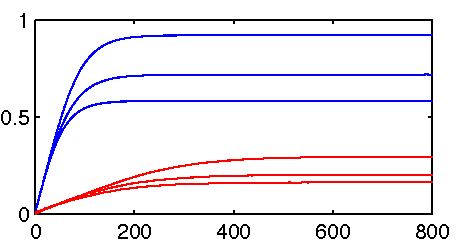
\includegraphics{history}\\
& time~$t$
\end{tabular}
\caption{The histories of the mean velocity $\bq$ for the flow over the straight channel~(blue) and meandering channel~(red) at three reasonable observed stations. 
The relevant parameters $2\beta=8$, $B=0.9$, $\kappa_1=1$, $\kappa_2=4\pi/L_x$, $\theta=0.01$~(straight) and $\theta=0.001$~(meander).
Zero slopes of these curves indicate the fluid converges to steady state. }
\label{history}
\end{figure}%

\begin{figure}[b]
\vspace{2mm}
\centering
\begin{tabular}{c@{}c}
\rotatebox{90}{\hspace{8ex} mean~$\uu$} &
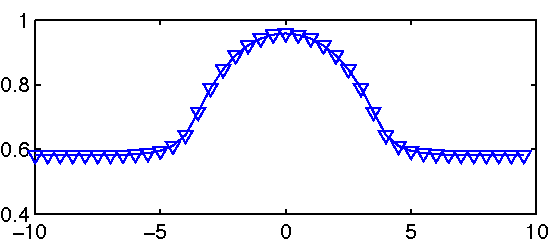
\includegraphics{straight-velocity-u}\\
& cross-section~$y$
\end{tabular}
\caption{Plot of the mean downstream velocity~$\uu$ in the cross-section at the point $x=20$ and the time $t=800$ with parameters $2\beta=8$, $B=0.9$ and $\theta=0.01$. 
The channel is nine times as deep in the middle as in the surrounding shallow regions, and the mean downstream velocity is one and a half times as fast in the middle as in the shallow regions.}
\label{straight-velocity-u}
\end{figure}%

\begin{figure}[b]
\vspace{2mm}
\centering
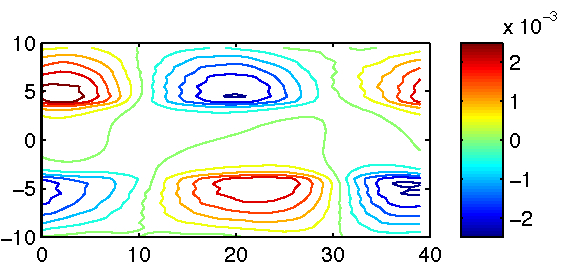
\includegraphics{straight-velocity-vc}
\caption{Contours of the mean transverse velocity~$\vv$ at time $t=800$ with parameters $2\beta=8$, $B=0.9$ and $\theta=0.01$. 
The high value curves~(red) and low value curves~(blue) indicate travelling vortices on the shear near the interactions between the channel and shallow regions. }
\label{straight-velocity-vc}
\end{figure}%

This section focuses on the application of the resulting model for turbulence flow over straight open channels. 
Consider the turbulence flow over a slightly sloping ground with a straight open channel. 
Compare this channel flow with small viscous open channel flow by Roberts et al.~\cite{Robertsli2006} and the experiments of turbulent flow over flood plains and channels in a flume with water of variable depth by Bousmar et al.~\cite{Bousmar2002,Bousmar2003a}. 
 
 Let~$x$ be the along stream coordinate,~$y$ be the horizontal distance across the stream on the channel and~$z$ be normal to the channel. 
Consider the water of a depth $h(x,y,t)$ flows with the mean lateral velocities $\uu(x,y,t)$ and $\vv(x,y,t)$ along the channel of
\begin{equation}
b(x,y)=-1+B-B\left[1-\left(\frac{y}{\beta}\right)^2\right]^2,\label{bed:straight}
\end{equation}
where~$\beta$ denotes the width of the channel, and~$B$ the mid-depth of the channel.  
The centreline of the channel locates at $y=0$.
Assume the channel has a width of  $2\beta=8$ and a slope $\theta=0.01$ in the $x$ direction.  
The mid-depth of the channel is $B=0.9$.
Consider the initial still water level is zero and then the depth of the shallow regions is $-1+0.9=-0.1$.
The channel of~\cite{Bousmar2002} is about two times as deep in the constant channel as in the flood plain.

Consider the fluid of zero initial water level flowing with small mean downstream velocity $\uu(x,y,t)$ down the open channel described by equation~\eqref{bed:straight}. 
Nondimensionalise the variables of fluid depth $h(x,y,t)$ and mean lateral velocities $\uu(x,y,t)$ and $\vv(x,y,t)$ with respect to some velocity scale, a typical depth and a fluid density, and consider $g=1$. 
Equations~\eqref{smag:h}--\eqref{smag:v} describe the dynamics of this fluid with the periodic boundary conditions both in the~$x$ and~$y$ directions for both the flow and channel. 

The flow in the simulation converges to steady state, shown by the blue curves in Figure~\ref{history}.
Figure~\ref{straight-velocity-u} shows that fast flow developed in the deeper channel and slow flow on the shallow regions.
This corresponds to the interpretation of Roberts et al.~\cite{Robertsli2006} for the viscous flow in a small open channel, where the viscous flow is eight times as fast in the channel as on the shallow regions. 
Equation~\eqref{smag:u} demonstrates the equilibrium downstream velocity in the shallow regions is $\sqrt{0.985\sin(0.01)*0.1/0.00293}=0.582$, which corresponds the numerical result in Figure~\ref{straight-velocity-u}. 
The equilibrium downstream velocity in the mid-channel should be $\sqrt{0.985\sin(0.01)*1/0.00293}=1.84$, but is~$0.95$ in the numerical simulation, shown in Figure~\ref{straight-velocity-u}. 
Numerical tests show that when the shape of the bed becomes complex, the equilibrium downstream velocity decreases. 
For example, for the slope~$\theta=0.001$, the equilibrium downstream velocity on the flat bed is~$0.582$, on the bed with straight channel with a width~$2\beta=14$ is~$0.374$, on the bed with straight channel with a width~$2\beta=8$ is~$0.302$, on the bed with slight meandering channel with a width~$2\beta=8$ is~$0.307$.
Figure~\ref{straight-velocity-vc} displays the contour of the mean transverse velocity~$\vv(x,y,t)$ at time~$t=800$, which indicates that weak horizontal vortices grow on the shear near the interactions between the channel and shallow regions, and travel downstream. 
Similar vortices were observed by~\cite{Robertsli2006} for the small viscous open channel flow and by~\cite{Bousmar2003a} for the turbulent flows over a flume. 

\begin{figure}[b]
\vspace{2mm}
\centering
\begin{tabular}{c@{}c}
\rotatebox{90}{\hspace{12ex}$y$}&
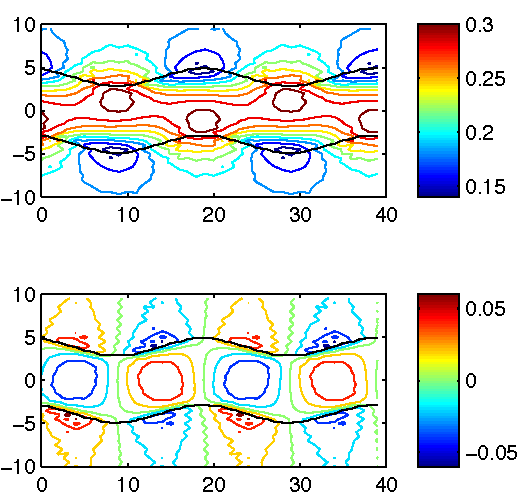
\includegraphics{meander-velocity-cont}\\
&$x$
\end{tabular}
\caption{Contours of the mean downstream velocity $\uu$~(top) and mean transverse velocity $\vv$~(bottom) at time $t=800$ with parameters $2\beta=8$, $B=0.9$, $\theta=0.01$, $\kappa_1=1$ and $\kappa_2=4\pi/L_x$. 
The black curves plot the meandering channel.}
\label{meander-velocity-cont}
\end{figure}%

\section{Modelling flows over meandering channels}

This part describes the simulations of turbulent fluid flowing over a slightly sloped ground with a meandering open channel. 
The simulations are compared with the numerical results of Liu et al.~\cite{Liu2009} and Demuren~\cite{Demuren1993} who calculated the two and three dimensional turbulence flows in meandering channels by a lattice Boltzmann model and a finite volume numerical model, respectively.

Create a Cartesian coordinate system~$(x,y,z)$ . 
Consider nondimensionalised fluid depth $h(x,y,t)$, mean lateral velocities $\uu(x,y,t)$ in the~$x$ direction and $\vv(x,y,t)$ in the~$y$ direction. 
Describe the meandering open channel~$b(x,y)$ by
\begin{align}&
b(x,y)=-1+B-B\left[1-\left(\frac{y-\kappa_1\cos(\kappa_2x)}{\beta}\right)^2\right]^2\,,\label{bed:meander}
\end{align}
where the parameter~$\kappa_1$ and~$\kappa_2$ determine the curvature of the meandering channel, and the parameters $\beta$ and~$B$ are the width and mid-depth of the meandering channel.
Simulate the turbulent flow over such channel by the equations~\eqref{smag:h}$--$\eqref{smag:v} with periodic boundary conditions in both~$x$ and~$y$ directions for both the flow and channel. 

\begin{figure}[b]
\centering
\begin{tabular}{c@{}c}
\rotatebox{90}{\hspace{8ex}depth~$h$} &
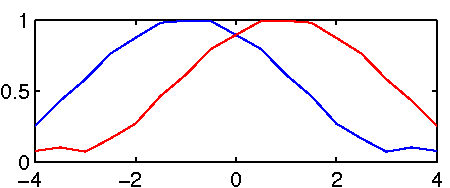
\includegraphics{meander-depth}\\
& channel~cross-section~$y$
\end{tabular}
\caption{Plot of the fluid depth $h(x,y,t)$ in the cross-section of the channel at stations~$x=10$~(blue) and~$x=20$~(red). 
The relevant parameters $2\beta=8$, $B=0.9$, $\theta=0.01$, $\kappa_1=1$ and $\kappa_2=4\pi/L_x$.}
\label{meander-depth}
\end{figure}%

The flow in the simulation converges to steady state, shown by the red curves in Figure~\ref{history}.
Figure~\ref{meander-velocity-cont} exhibit the contours of the mean lateral velocities $\uu(x,y,t)$ and $\vv(x,y,t)$. 
The mean downstream velocity~$\uu$ reaches maximum at the bends.
The mean transverse velocity~$\vv$ gets to maximum and minimum at the connection of the bends, which are consistent with the results of Liu eta al.~\cite{Liu2009} who modelled the water in meandering channels with~$60^\circ$ and~$90^\circ$ consecutive bends and a width of~$0.3$\,m.
Demuren~\cite{Demuren1993} calculated the depth and the depth-averaged longitudinal and transverse velocities of three dimensional flows in meandering channels with natural bed configuration by a finite volume numerical method. 
Simulations at fifteen observed stations of the meandering channel indicate that the location of the maximum velocity shifts from the inner bank to the outer bank as the water flowing through the bends of the channel. 
Figure~\ref{meander-depth} and~\ref{meander-velocity} show the plots of the depth $h(x,y,t)$, the mean downstream velocity $\uu(x,y,t)$ and the mean transverse velocity $\vv(x,y,t)$ at the channel bends $x=10$ and $x=20$.
The depth, downstream velocity and transverse velocity are bigger in the outer bank than in the inner bank, which correspond to the computations by Demuren~\cite{Demuren1993}. 


\begin{figure}[b]
\vspace{2mm}
\centering
\begin{tabular}{c@{}c}
\rotatebox{90}{\hspace{7ex}mean lateral velocities~$\uu$~and~$\vv$} &
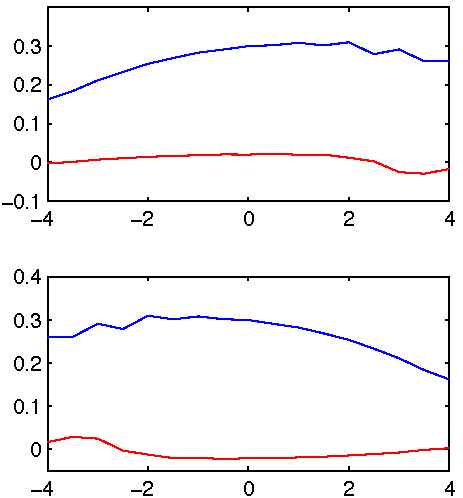
\includegraphics{meander-velocity}\\
& channel~cross-section~$y$\\
\end{tabular}
\caption{Plots of the mean downstream velocity $\uu(x,y,t)$~(blue) and the mean transverse velocity $\vv(x,y,t)$~(red) in the cross-section of the channel at the bend $x=10$~(top) and $x=20$~(bottom). 
The relevant parameters $2\beta=8$, $B=0.9$, $\theta=0.01$, $\kappa_1=1$ and $\kappa_2=4\pi/L_x$.}
\label{meander-velocity}
\end{figure}%

\section{Conclusion}

The proposed approach supporting by centre manifold theory describes the environmental turbulent fluids reliably. 
The flows in straight and meandering compound channel, as examples, are simulated by the new approach. 
The results correspond to the analysis and numerical simulations of the published work~\cite[e.g.]{Bousmar2002,Liu2009}.
 The equations~\eqref{smag:h}--\eqref{smag:v} account for the interactions between the vertical profiles and lateral spatial variations, and thus can be used to predict erosion and sand transport of the turbulent fluid in the further work.




\bibliographystyle{afmc}
\bibliography{bibsmag}
\end{document}